\documentclass[11pt,a4paper,oneside]{book}
%
%--------------------   start of the 'preamble'
%
\usepackage[table]{xcolor}
\usepackage{graphicx,amssymb,amstext,amsmath,float,color,array,ctable,booktabs,wrapfig,caption}
%


\usepackage{filecontents}
\begin{filecontents}{ref.bib}
@article{li2008mapping,
  title={Mapping short DNA sequencing reads and calling variants using mapping quality scores},
  author={Li, Heng and Ruan, Jue and Durbin, Richard},
  journal={Genome research},
  volume={18},
  number={11},
  pages={1851--1858},
  year={2008},
  publisher={Cold Spring Harbor Lab}
}

@article{Kivioja:2012kg,
author = {Kivioja, Teemu and V{\"a}h{\"a}rautio, Anna and Karlsson, Kasper and Bonke, Martin and Enge, Martin and Linnarsson, Sten and Taipale, Jussi},
title = {{Counting absolute numbers of molecules using unique molecular identifiers.}},
journal = {Nature methods},
year = {2012},
volume = {9},
number = {1},
pages = {72--74},
month = jan
}


@book{durbin,
    author = {Durbin, R. and Eddy, S. and Krogh, A. and Mitchison, G.},
    edition = {eleventh},
publisher = {Press, Cambridge U.},
    title = {{Biological sequence analysis}},
    year = {2006}
}



@article{Kall:2005vg,
author = {K{\"a}ll, Lukas and Krogh, Anders and Sonnhammer, Erik L L},
title = {{An HMM posterior decoder for sequence feature prediction that includes homology information}},
journal = {Bioinformatics (Oxford, England)},
year = {2005}
}

\end{filecontents}

\usepackage{graphics}
\usepackage{hyperref}
\usepackage{pgf}
\usepackage{natbib}
\usepackage{verbatim}
\usepackage{titlesec}
\titleformat{\chapter}[hang] 
{\normalfont\huge\bfseries}{\ \thechapter}{1em}{} 
\usepackage{tikz}
\usetikzlibrary{shapes}
\usetikzlibrary{calc,backgrounds}
\usetikzlibrary{automata}
\usetikzlibrary{arrows,positioning,calc,matrix} 
\usetikzlibrary{decorations.pathreplacing,shapes.multipart}

\tikzstyle{Dstate}=[shape=circle,draw=black!50,fill=black!10]
\tikzstyle{Istate}=[shape=diamond,draw=black!50,fill=black!10]
\tikzstyle{Mstate}=[shape=rectangle,draw=black!50,fill=black!10]

\tikzstyle{empty}=[shape=circle]

\tikzstyle{lightedge}=[->,dotted,thick]
\tikzstyle{mainstate}=[state,thick]
\tikzstyle{mainedge}=[->,thick]

\definecolor{black}{RGB}{0,0,0}
\definecolor{darkgrey}{RGB}{64,64,64}
\definecolor{grey}{RGB}{127,127,127}
\definecolor{lightgrey}{RGB}{230,230,230}

% scheme 1 
\definecolor{winered}{RGB}{158,16,0}
\definecolor{lightred}{RGB}{199,53,42}
\definecolor{brown}{RGB}{158,95,0}
\definecolor{orange}{RGB}{235,141,0}

%scheme2

\definecolor{darkblue}{RGB}{19,48,182}

\definecolor{blue}{RGB}{36,89,158}
\definecolor{browngreen}{RGB}{82,75,19}
\definecolor{lightbrown}{RGB}{158,126,36}

%scheme3

\definecolor{green}{RGB}{52,132,23}


\definecolor{lightgreen}{RGB}{82,209,36}
\definecolor{lightbrowngreen}{RGB}{125,133,23}
\definecolor{yellowgreen}{RGB}{198,209,36}

%scheme4


\definecolor{paper}{RGB}{240,238,183}
\definecolor{organicgrey}{RGB}{163,162,124}


\definecolor{metal}{RGB}{75,81,82}


\setlength{\parindent}{0cm}
\pagestyle{empty}

\makeindex
\usepackage{anysize}

%\marginsize{left}{right}{top}{bottom}:
\marginsize{2cm}{2cm}{2cm}{2cm}

\begin{document}
\frontmatter
%-----------------------------------------------------------
\newlength{\centeroffset}
%\setlength{\centeroffset}{-0.5\oddsidemargin}
%\addtolength{\centeroffset}{0.5\evensidemargin}
%\addtolength{\textwidth}{-\centeroffset}
\thispagestyle{empty}
\vspace*{\stretch{1}}
\noindent\hspace*{\centeroffset}\makebox[0pt][l]{\begin{minipage}{\textwidth}
\flushright
{\Huge\bfseries 

The TagDust2 Manual

}


\end{minipage}}

\vspace{\stretch{1}}
\noindent\hspace*{\centeroffset}\makebox[0pt][l]{\begin{minipage}{\textwidth}
\flushright


\vspace{\stretch{1}}
{\bfseries 
by Timo Lassmann\\[1.5ex]} 
\noindent\rule[-1ex]{\textwidth}{1pt}\\[2.5ex]
 \today

\end{minipage}}

%\addtolength{\textwidth}{\centeroffset}
%\vspace{\stretch{2}}


\pagebreak
\begin{small} 

Copyright \copyright  2013, 2014 Timo Lassmann (timolassmann@gmail.com)
 
 This document is free;  you can redistribute it and/or modify
 it under the terms of the GNU General Public License as published by
 the Free Software Foundation, either version 3 of the License, or
 (at your option) any later version.
 
 This document is distributed in the hope that it will be useful,
 but WITHOUT ANY WARRANTY; without even the implied warranty of
 MERCHANTABILITY or FITNESS FOR A PARTICULAR PURPOSE.  See the
 GNU General Public License for more details.
 
 You should have received a copy of the GNU General Public License
 along with TagDust.  
 
 If not, see (http://www.gnu.org/licenses/).



\end{small}

%-----------------------------------------------------------
\tableofcontents
%-----------------------------------------------------------
\mainmatter
%\setcounter{chapter}{-1}

%\setcounter{chapter}{1}
%\setcounter{section}{0}
\chapter{Introduction}

 %\addcontentsline{toc}{chapter}{Introduction}

Raw sequences produced by next generation sequencing (NGS) machines can contain adapter, linker, barcode and fingerprint sequences. TagDust2 is a program to extract and correctly label the sequences to be mapped in downstream pipelines.

TagDust allows users to specify the expected architecture of a read and converts it into a hidden Markov model. The latter can assign sequences to a particular barcode (or index) even in the presence of sequencing errors. Sequences not matching the architecture (primer dimers, contaminants etc.) are automatically discarded (see Figure \ref{figure1}).


%\begin{wrapfigure}{l}{1\textwidth}

\begin{figure}[h!]

\begin{center}
\includegraphics[scale = 0.7]{figures/figure1.pdf}
\end{center}
\caption{A HMM specifies the expected architecture of the raw sequence. After decoding sequences are segmented into the components of the architecture. Based on the segmentation, a barcode is assigned to each read and remaining sequences are trimmed.}
\label{figure1}
\end{figure}


%\end{wrapfigure}

\newpage

\chapter{Installation}
%\addcontentsline{toc}{chapter}{Installation}


%\section*{Quick installation instructions}
%\addcontentsline{toc}{section}{Quick installation instructions}
Unpack the tarball:

\begin{verbatim}
bash-3.1$ tar -zxvf tagdust-2.04.tar.gz 
\end{verbatim}

\begin{verbatim}
bash-3.1$ cd tagdust
\end{verbatim}


\begin{verbatim}
bash-3.1$ ./configure
\end{verbatim}
\begin{verbatim}
bash-3.1$ make
\end{verbatim}

\begin{verbatim}
bash-3.1$ make check
\end{verbatim}
At this point the TagDust executable appears in the src/ directory. You can copy it to any directory in your path. To install it system wide type:  
\begin{verbatim}
bash-3.1$ make install
\end{verbatim}
%\let\clearpage\relax
\chapter{Quick Usage}

\section{Single-end data}

Simply:

\begin{verbatim}
bash-3.1$ tagdust -arch architectures.txt in.fq -o output
\end{verbatim}

The file ``architectures.txt'' needs to contain at least one valid tagdust architecture. For example: 


\begin{verbatim}
bash-3.1$ more architectures.txt

./tagdust -1 B:AAA,TTT -2 R:N 
\end{verbatim}

In the case above TagDust will try to split the input reads into those containing either AAA or TTT barcodes at the start of the raw reads. 

\section{Paired-end data}

Simply:

\begin{verbatim}
bash-3.1$ tagdust -arch architectures.txt read1.fq read2.fq -o output
\end{verbatim}
 

\chapter{Usage}

\section{Command Line}
TagDust requires an input file containing sequences and a user specified HMM architecture used to extract the reads. For the architecture all that TagDust needs to know is the sequence of pre-defined building blocks. Options '{\tt -1,-2, ...}' are used to specify the first, second, etc. building block. Alternatively the architecture(s) can be supplied in a separate input file using the -arch option (see section \ref{arch}).  

\begin{verbatim}
bash-3.1$ tagdust <options> <read1.fq>  [read2.fq] -o <output prefix> 
\end{verbatim}

\rowcolors{1}{lightgrey}{white}

\begin{center}
\begin{tabular}{| l | l | p{12cm}|}
\hline
\rowcolor{blue} \textcolor{white}{\scshape Option}		&\textcolor{white}{\scshape Type}		&	\textcolor{white}{\scshape Description}\\ \hline
%-start & INT & start of search area [0].\\
%-end & INT & end of  search area [length of sequence].\\
-arch & STR & path and name of file containing tag dust architectures. \\
%-format & STR & format of input sequence file.\\
-minlen & INT & minimal accepted read length [16].\\
-ref     &  STR &    reference fasta file to be compared against[].\\
-fe &       INT &    number of errors allowed when comparing to reference[2].\\
-dust &	INT &	remove low complexity sequences[].\\
%-e & FLT & expected sequencer error rate [0.05].\\ 
-o & STR & output prefix.\\
%-a & STR & output file for artifacts [NA].\\
-t & INT & number of threads [8].\\
-1 & STR & type of the first HMM building block. \\
-2 & STR & type of the second HMM building block.\\
-\dots & STR & type of the \dots HMM building block.\\
\hline
\end{tabular}
\end{center}

If two fast files are given TagDust assumes the input is a paired end library.

\vspace{10 mm}


Here are some examples of HMM building blocks:
\begin{center}


\begin{tabular}{| l | l | p{12cm}|}
\hline
\rowcolor{blue} \textcolor{white}{\scshape Example}		&\textcolor{white}{\scshape Type}		&	\textcolor{white}{\scshape Description}\\ \hline
R:N & Read  & a block containing a read to be extracted.\\
S:AATT & Spacer & a block containing the sequence AATT.\\ 
B:ACT,GGG & Barcode/Index & a three nucleotide long block containing either ACT or GGG\\ 
F:NNNNNN & Fingerprint / UMI & a six nucleotide long {\bf U}nique {\bf M}olecular {\bf I}dentifier.\\ 
O:T  & Optional & a block modeling the optimal inclusion of a single or multiple Ts.\\
\hline
\end{tabular}
\end{center}

Also have a look at the more detailed description further down and the usage examples. 


\newpage 
\section{Output}
TagDust will split the input file(s) into several output files. The number and names of output files depend on the type of library: 


\begin{center}
\begin{tabular}{ | c | p{4.5cm} | p{4.5cm}|}
\hline
 \textcolor{white}{\scshape }		&\cellcolor{blue}\textcolor{white}{\scshape No barcodes}		&	\cellcolor{blue}\textcolor{white}{\scshape Barcodes}\\ \hline
\cellcolor{blue}\textcolor{white}{\scshape Single End} & $<$p$>$.fq \newline $<$p$>$\_un.fq & $<$p$>$\_BC\_GTA.fq $<$p$>$\_BC\_AAA.fq $<$p$>$\_BC\_\dots.fq \newline $<$p$>$\_un.fq \\
\cellcolor{blue}\textcolor{white}{\scshape Paired End} &  $<$p$>$\_READ1.fq $<$p$>$\_READ2.fq $<$p$>$\_un\_READ1.fq $<$p$>$\_un\_READ2.fq   & $<$p$>$\_BC\_GTA\_READ1.fq $<$p$>$\_BC\_GTA\_READ2.fq  $<$p$>$\_BC\_AAA\_READ1.fq $<$p$>$\_BC\_AAA\_READ2.fq $<$p$>$\_BC\_\dots\_READ1.fq $<$p$>$\_BC\_\dots\_READ2.fq $<$p$>$\_un\_READ1.fq $<$p$>$\_un\_READ2.fq\\ 
\hline
\end{tabular}
\end{center}
$<$p$>$ is the prefix specified by the -o option. ``{\bf BC}'' stands for barcode and ``{\bf un}'' for un-extracted reads. All auxiliary sequences such as spacers, barcodes are removed from the sequences in the output files. 

In addition TagDust summarizes key information about the run in a log file named $<$p$>$\_logfile.txt. For example:
	
{\small
\begin{verbatim}
[2014-05-15 16:18:05]   Tagdust 2.10, Copyright (C) 2013 Timo Lassmann
[2014-05-15 16:18:05]   cmd: tagdust-2.10/src/tagdust -arch arch.txt -t 80 
-o all_demultiplexed all_raw.fq 

[2014-05-15 16:18:05]   Start Run
--------------------------------------------------
[2014-05-15 16:18:05]   Running in single end mode.
[2014-05-15 16:18:05]   Searching for best architecture in file 'arch.txt'
[2014-05-15 16:18:07]   Using: -1 O:N -2 B:TTTAGG,ATTCCA,GCTCAA,CATCCC  -3 S:GGG -4 R:N 
[2014-05-15 16:18:07]   Confidence: 1.00
[2014-05-15 16:18:39]   Long sequence found. Need to realloc model...
[2014-05-15 16:21:11]   Selected Threshold:: 1.636996
[2014-05-15 22:24:06]   Done.

[2014-05-15 22:24:07]   all_raw.fq      Input file name.
[2014-05-15 22:24:07]   110622138       total input reads
[2014-05-15 22:24:07]   1.64    selected threshold
[2014-05-15 22:24:07]   100699341       successfully extracted
[2014-05-15 22:24:07]   91.0%   extracted
[2014-05-15 22:24:07]   2529699 problems with architecture
[2014-05-15 22:24:07]   42906   barcode / UMI not found
[2014-05-15 22:24:07]   0       too short
[2014-05-15 22:24:07]   7350192 low complexity
[2014-05-15 22:24:07]   0       match artifacts
\end{verbatim}
}

\section{Notes}
%\subsection{Threshold}
%The {\tt -Q} option sets the minimum acceptable read quality analogous to the mapping quality Q. If the reads are very short or the model very simple (e.g. 3 nucleotide barcode followed by the read) the default threshold of 20 might have to be lowered.

%\subsection{Logfile}
%The log option ({\tt -l} flag) specifies the directory into which log files will be written. The log file name is the input file name and the suffix  "\_tagdust\_log.txt". It contains some basic statistics on the number of reads making it through the various TagDust steps. It also lists the number of matches to known contaminants (see below).  

\subsection{Removing Known Contaminants (e.g. ribosomal RNA sequences).}
Known contaminants or unwanted reads can be filtered from the output by pointing TagDust to a reference fasta to be matched against ({\tt -ref <filename>} ). The maximum number of errors allowed for a match to reference is set with the {\tt -fe} option. {\bf In the current implementation only the first 32 nucleotides off the extracted read are compared against the reference sequences!}
\subsection{Removing Low Complexity Sequences}
Tagdust implements a simplified version of the DUST module (R. Tatusov and D.J. Lipman, unpublished data) to filter out low complexity reads. While this is not strictly necessary for NGS reads I implemented it to remove poly-A and other "very" low complexity sequences. The algorithm is only applied to the first 64 nucleotides of the reads. The {\tt -dust} option both enables and sets the threshold for the low complexity filtering. I recommend using a relaxed threshold of 100 and leave the rest to the downstream mapping algorithm. 


\subsection{Efficiency}
As a default, TagDust attempts to match the entire sequence to the HMM (global). The options {\tt -start} and {\tt -end} restricts the matching to region specified. TagDust assumes that all residues upstream of 'start' do not belong to the read while all residues following 'end' are read residues.



%\subsection{Extracting multiple reads from a  single input read}

%If a user specified architecture contains multiple read segments (e.g. -1 R:N -2 S:TTTTTT -3 R:N) TagDust will print out multiple reads per input. The tag {\bf RS:$1...X$} is appended to the raw read name to distinguish the reads.


\section{Formats}
\subsection{Input file formats}

TagDust can work with fasta, fastq and SAM/BAM files. Gzipped files are also supported. The format is automatically recognized by the file suffix. %If the input is streamed, the '{\tt -format}' option has to be used to specify the format.\\
 
%\subsection{Output format}
%The output format is always a fastq file. If barcodes or fingerprints are present, TagDust appends them to the read name: 

%{\small
%\begin{verbatim}
%@110922_SN549_0034_BB03F7ABXX:7:1101:1137:1974#0/1 BC:AGT;FP:367
%CNCTGAAACGTAGATATAGGGGAACCCCGCCTGTTTACCAAAAACATCACCTCTAGCAT
%+
%bBS`cceegggggiiiiiiiiiiiiiiiiiiiihhihhhiihhhiiihiiihiiiiggg
%\end{verbatim}
%}

%Note that BC:[A,C,G,T]+ is the sequence of the barcode and FP:[0-9]+ is the fingerprint sequence converted into a unique decimal number.

%If multiple reads are present TagDust appends the tag {\tt RS:X} to the read name: 

%{\small
%\begin{verbatim}
%@110922_SN549_0034_BB03F7ABXX:7:1101:1137:1974#0/1 BC:AGT;FP:367;RS:1 
%CNCTGAAACGTAGATATAGGGGAACCCCGCCTGTTTACCAAAAACATCACCTCTAGCAT
%+
%bBS`cceegggggiiiiiiiiiiiiiiiiiiiihhihhhiihhhiiihiiihiiiiggg
%
%\end{verbatim}
%}
 

\section{Examples: putting it all together}

Here are some examples: 

\subsection{A library containing both barcodes and a 8 nucleotide fingerprint.}

In this example we expect the sequenced reads to contain a 6 nucleotide barcode sequence (out of a selection of 8) followed by a 8 nucleotide fingerprint, followed by the spacer sequence `TATA` followed by the read. \\

Here is the corresponding TagDust command: 


{\small
\begin{verbatim}
bash-3.1$ tagdust test.fq.gz   -1 O:N -2 B:ACAGAT,ATCGTG,CACGAT,CACTGA,CTGACG,GAGTGA,GTATAC,TCGAGC
-3 F:NNNNNNNN -4 S:TATA -5 R:N  -o output.fq
\end{verbatim}
}

Note that we added an optional state at the beginning of the read in case extra nucleotides were added before the barcode.  \\ 

To remove ribosomal reads simply add the -ref and -fe options:

{\small
\begin{verbatim}
bash-3.1$ tagdust test.fq.gz   -1 O:N -2 B:ACAGAT,ATCGTG,CACGAT,CACTGA,CTGACG,GAGTGA,GTATAC,TCGAGC
-3 F:NNNNNNNN -4 S:TATA -5 R:N  -o output.fq -ref U13369.1.fa -fe 2 
\end{verbatim}
}




\subsection{A RNA-seq library with a 'spaced' fingerprint.}

Here I downloaded a dataset from \cite{Kivioja:2012kg}. Reads start after the following construct:

{
\begin{verbatim}
(NNN)dU(NNNN)dU(NNN)[GACTT]rGrGrGrG
\end{verbatim}
}
dU and rG represent deoxyuridine and guanine ribonucleotide, respectively. N's in brackets are the fingerprint nucleotides while GACTT is the barcode used. As you can see the ten nucleotide fingerprint is split into 3 parts separated by T's. \\

Here is the corresponding TagDust command: 


{\small
\begin{verbatim}

bash-3.1$ tagdust ERR048990.fastq  -1 F:NNN -2 S:T -3 F:NNNN -4 S:T -5 F:NNN -6 B:GACTT
-7 S:GGGG -8 R:N -start 1 -end 25  -o output.fq
\end{verbatim}
}

Note on the last line I restricted the search to the first 25 nucleotides for efficiency. 


\subsection{Extracting multiple reads from a single input.}

Here is a simulated case where we have reads at the 5' and 3' end of the input read separated by {\tt GGGGGGGGAAAAAAAA}:

\vspace{10 mm}

{\small
%\begin{verbatim}
\tt @SRR1043305.1 RunXXXXX 

{\color{red}ATTGCTGTCTCTTATACACATC}GGGGGGGGAAAAAAAA{\color{blue}TGACGCTGCCCAGATCGTATGCCGTCTTC}

+

\_\_bccceefaeeefhfhhhhfhdddhhhaghhhdgffgfYffghfd\_cffhffffffffffffffff

@SRR1043305.2 RunXXXXX 

{\color{red}GATCGGGGGAACTTTCAGGATC}GGGGGGGGAAAAAAAA{\color{blue}TGTCTCTTATACACATCTGACGCTGCCCA}

+

bb\_eeeeegfgegiiiiiihhhieffhhfhiihhhffhhifiifiiggbedffffffffffffffff

%\end{verbatim}
}

\vspace{10 mm}

To extract the reads: 
\vspace{10 mm}

{\small
\begin{verbatim}
bash-3.1$ tagdust test.fq -1 R:N -2 S:GGGGGGGGAAAAAAAA -3 R:N -o out
\end{verbatim}
}

The original reads will be split among two output files: 

\begin{center}
\begin{tabular}{|p{7cm}|p{7cm}|}
\hline \rowcolor{blue} \textcolor{white}{ out\_READ1.fq} & \textcolor{white}{ out\_READ2.fq} \\
{\small \tt @SRR1043305.1 RunXXXXX \newline {\color{red}ATTGCTGTCTCTTATACACATC}  \newline + \newline \_\_bccceefaeeefhfhhhhfh  \newline @SRR1043305.2 RunXXXXX  \newline {\color{red}GATCGGGGGAACTTTCAGGATC}  \newline +  \newline bb\_eeeeegfgegiiiiiihhh}
  & 
  {\small  \tt @SRR1043305.1 RunXXXXX  \newline {\color{blue}TGACGCTGCCCAGATCGTATGCCGTCTTC}  \newline + \newline fYffghfd\_cffhffffffffffffffff  \newline
@SRR1043305.2 RunXXXXX  \newline {\color{blue}TGTCTCTTATACACATCTGACGCTGCCCA}  \newline +  \newline  hifiifiiggbedffffffffffffffff }\\  \hline
\end{tabular}
\end{center}

\subsection{Using the -arch option}\label{arch}

When TagDust is given an architecture file containing multiple architectures it will scan a proportion of the  input data with all architectures and automatically select the best matching one. For example, the file below contains three architectures:

\vspace{5mm}

{\small \tt
tagdust -1 B:TGCT,AAAA,AACC,AAGG,AATT,ACAC,ACCA,ACGT -2 R:N in.fq -o out.fq \\
tagdust -1 P:agggaggacgatgcgg -2 B:TGCT,AAAA,AACC,AAGG,AATT,ACAC,ACCA,ACGT -3 R:N \\ -4 P:gtgtcagtcacttccagcgg in.fq -o out.fq\\
tagdust -1 P:agggaggacgatgcgg -2 B:TGCT,AAAA,AACC,AAGG,AATT,ACAC,ACCA,ACGT,ACTG,AGAG,AGGA\\,AGTC,ATAT,ATCG,ATGC,ATTA,CAAC,CACA,CAGT,CATG,CCAA,CCCC,CCGG,CCTT -3 R:N \\ -4 P:gtgtcagtcacttccagcgg in.fq -o out.fq\\
}

\vspace{5mm}

Tagdust will scan the file looking for the keyword ``tagdust'' and assume the remaining words in the line are parameters. 

The first two architectures contain eight barcodes / indices but the second one additionally assumes the presence of 5' and 3' linkers. The third architecture assumes the presence of 24 barcodes and linkers. When running: 

\begin{verbatim}
bash-3.1$ tagdust -arch architectures.txt in.fq -o output
\end{verbatim}

TagDust will automatically select the correct architecture and proceed as normal. 

When the input is paired-end data, TagDust will scan both input files with all architectures and attempt to find a match for both reads. {\bf If a match is found for only one file, TagDust will assume the file only contains valid reads. }



\newpage

\chapter{HMM Building Blocks}
TagDust comes with a set of pre-defined HMM building blocks. Each includes a silent state at the beginning and end used to link blocks together. Each block is specified by a unique letter following by a colon and some information about the sequence. 


\section{Read}
Segment modeling the read. \\

\begin{figure}[H]
\centering
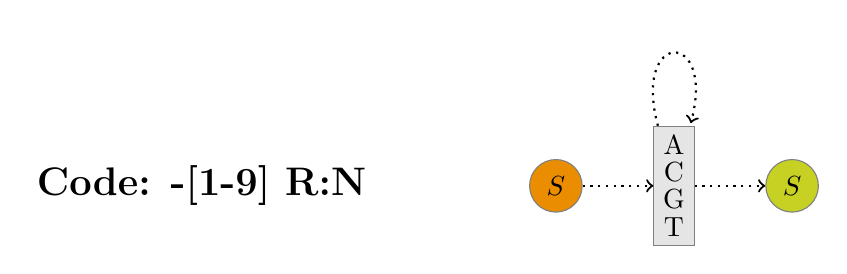
\begin{tikzpicture}
 
  \node  at (-6,0)  [font=\Large,style={align=center}] () {{\bf Code: -[1-9] R:N}};
 
\node[Dstate,fill=orange] (START) at (-1.5,0){$S$};

\node[Mstate] (O1) at (0,0){\shortstack{ A\\   C\\  G\\ T} };

\node[Dstate,fill=yellowgreen] (END) at (1.5,0){$S$};

 \path 

(START) edge [lightedge] (O1) 
(O1) edge [lightedge] (END) 

   
(O1) edge [lightedge,loop above] ();

\end{tikzpicture}
\end{figure}

\section{Optional}
Segment modeling an optional single or short stretch of nucleotides.  \\
Example code: O:N\\


\begin{figure}[H]
\centering
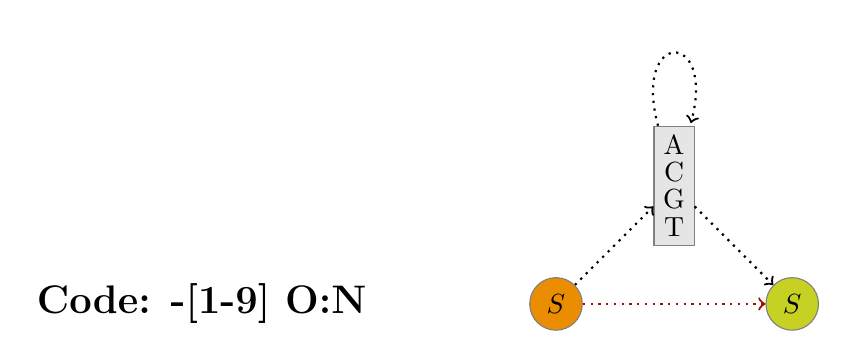
\begin{tikzpicture}
 
 \node  at (-6,0)  [font=\Large,style={align=center}] () {{\bf Code: -[1-9] O:N}};
 
\node[Dstate,fill=orange] (START) at (-1.5,0){$S$};

\node[Mstate] (O1) at (0,1.5){\shortstack{ A\\   C\\  G\\ T} };

\node[Dstate,fill=yellowgreen] (END) at (1.5,0){$S$};

 \path 

(START) edge [lightedge] (O1) 
(O1) edge [lightedge] (END) 
(START) edge [winered,lightedge] (END)
   
(O1) edge [lightedge,loop above] ();

\end{tikzpicture}
\end{figure}

\newpage
\section{G addition}
Segment modeling the occasional addition of guanines to the reads. (89.3\% chance of a single G , 19.5 \% chance of  2 Gs..).\\
Example code: O:N\\


\begin{figure}[H]
\centering
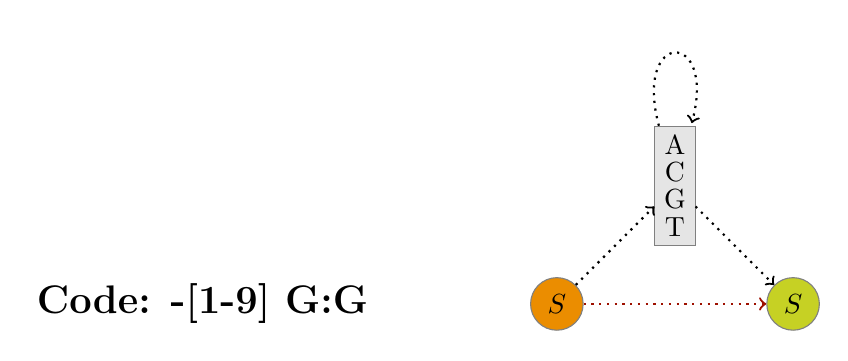
\begin{tikzpicture}
 
 \node  at (-6,0)  [font=\Large,style={align=center}] () {{\bf Code: -[1-9] G:G}};
 
\node[Dstate,fill=orange] (START) at (-1.5,0){$S$};

\node[Mstate] (O1) at (0,1.5){\shortstack{ A\\   C\\  G\\ T} };

\node[Dstate,fill=yellowgreen] (END) at (1.5,0){$S$};

 \path 

(START) edge [lightedge] (O1) 
(O1) edge [lightedge] (END) 
(START) edge [winered,lightedge] (END)
   
(O1) edge [lightedge,loop above] ();

\end{tikzpicture}
\end{figure}



\section{Barcode or Index}

Segment modeling a set of barcode sequences. For each sequence a separate HMM is created. The barcode sequences must be given as a comma separated list. A null model of the same length as the barcode is automatically added and initialized to the background nucleotide frequencies. \\



\begin{figure}[H]
\centering
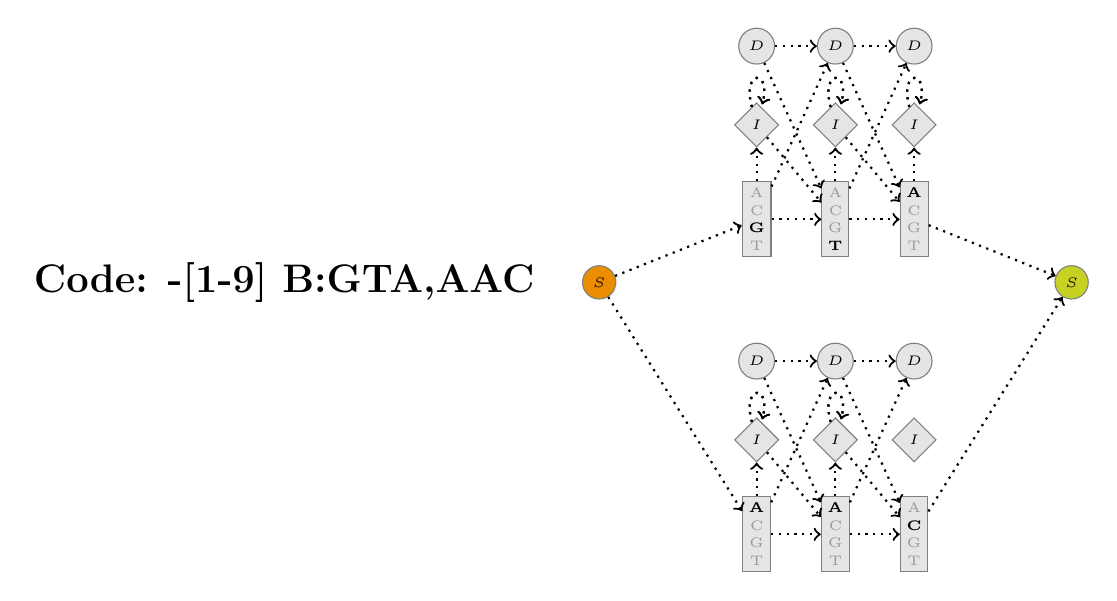
\begin{tikzpicture}
 \tiny
 
 \node  at (-7,0)  [font=\Large,style={align=center}] () {{\bf Code: -[1-9] B:GTA,AAC}};
 
 \node[Dstate,fill=orange] (START) at (-3,0){$S$};
 
\node[Dstate,fill=yellowgreen] (END) at (3,0){$S$};
 
\begin{scope}[shift={(-1,2)}];
\node[Dstate] (d1) at (0,1){$D$};
\node[Istate] (i1) at (0,0){$I$};
\node[Mstate] (m1) at (0,-1.2){\shortstack{ {\color{black!40}A}\\   {\color{black!40}C}\\  {\bf G}\\   {\color{black!40}T}} };



\node[Dstate] (d2) at (1,1){$D$};
\node[Istate] (i2) at (1,0){$I$};
\node[Mstate] (m2) at (1,-1.2){\shortstack{ {\color{black!40}A}\\   {\color{black!40}C}\\   {\color{black!40}G}\\   {\bf T}} };


\node[Dstate] (d3) at (2,1){$D$};
\node[Istate] (i3) at (2,-0){$I$};
\node[Mstate] (m3) at (2,-1.2){\shortstack{ {\bf A}\\   {\color{black!40}C}\\   {\color{black!40}G}\\   {\color{black!40}T}} };
\end{scope}


\begin{scope}[shift={(-1,-2)}];

\node[Dstate] (d4) at (0,1){$D$};
\node[Istate] (i4) at (0,0){$I$};
\node[Mstate] (m4) at (0,-1.2){\shortstack{ {\bf A}\\   {\color{black!40}C}\\   {\color{black!40}G}\\   {\color{black!40}T}} };



\node[Dstate] (d5) at (1,1){$D$};
\node[Istate] (i5) at (1,0){$I$};
\node[Mstate] (m5) at (1,-1.2){\shortstack{ {\bf A}\\   {\color{black!40}C}\\   {\color{black!40}G}\\   {\color{black!40}T}} };


\node[Dstate] (d6) at (2,1){$D$};
\node[Istate] (i6) at (2,-0){$I$};
\node[Mstate] (m6) at (2,-1.2){\shortstack{ {\color{black!40}A}\\   {\bf C}\\   {\color{black!40}G}\\   {\color{black!40}T}} };
\end{scope}

\path
(START)  edge [lightedge] (m1) 
(START)  edge [lightedge] (m4) 

(m3)  edge [lightedge] (END) 
(m6)  edge [lightedge] (END) 
(m1) edge [lightedge] (m2) 
(m1) edge [lightedge] (d2) 
(m1) edge [lightedge] (i1)
   
(i1) edge [lightedge,loop above] ()
(i1) edge  [lightedge] (m2)
(i1) edge [lightedge, loop above] ()
(d1) edge  [lightedge,->] (d2)
(d1) edge  [lightedge,->] (m2)

(m2) edge [lightedge] (m3) 
(m2) edge [lightedge] (d3) 
(m2) edge [lightedge] (i2)
   
(i2) edge [lightedge,loop above] ()
(i2) edge  [lightedge] (m3)
(i2) edge [lightedge, loop above] ()
(d2) edge  [lightedge,->] (d3)
(d2) edge  [lightedge,->] (m3)


(m3) edge [lightedge] (i3)
   
(i3) edge [lightedge,loop above] ()

(i3) edge [lightedge, loop above] ()


(m4) edge [lightedge] (m5) 
(m4) edge [lightedge] (d5) 
(m4) edge [lightedge] (i4)
   
(i4) edge [lightedge,loop above] ()
(i4) edge  [lightedge] (m5)
(i4) edge [lightedge, loop above] ()
(d4) edge  [lightedge,->] (d5)
(d4) edge  [lightedge,->] (m5)

(m5) edge [lightedge] (m6) 
(m5) edge [lightedge] (d6) 
(m5) edge [lightedge] (i5)
   
(i5) edge [lightedge,loop above] ()
(i5) edge  [lightedge] (m6)
(i5) edge [lightedge, loop above] ()
(d5) edge  [lightedge,->] (d6)
(d5) edge  [lightedge,->] (m6);



\end{tikzpicture}
\end{figure}
\newpage
\section{Fingerprint or {\underline U}nique {\underline M}olecular {\underline I}dentifier - UMI}

Segment modeling a fingerprint (or unique molecular identifiers). Insertions and deletions are by default not allowed within a fingerprint segment.

\begin{figure}[H]
\centering
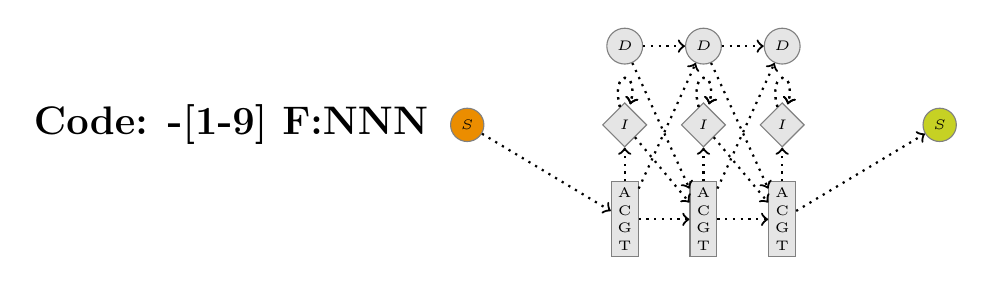
\begin{tikzpicture}
 \tiny
 
  \node  at (-6,0)  [font=\Large,style={align=center}] () {{\bf Code: -[1-9] F:NNN}};
 \node[Dstate,fill=orange] (START) at (-3,0){$S$};
 
\node[Dstate,fill=yellowgreen] (END) at (3,0){$S$};
 
\begin{scope}[shift={(-1,0)}];
\node[Dstate] (d1) at (0,1){$D$};
\node[Istate] (i1) at (0,0){$I$};
\node[Mstate] (m1) at (0,-1.2){\shortstack{ A\\   C\\  G\\ T} };



\node[Dstate] (d2) at (1,1){$D$};
\node[Istate] (i2) at (1,0){$I$};
\node[Mstate] (m2) at (1,-1.2){\shortstack{ A\\   C\\  G\\ T}};


\node[Dstate] (d3) at (2,1){$D$};
\node[Istate] (i3) at (2,-0){$I$};
\node[Mstate] (m3) at (2,-1.2){\shortstack{ A\\   C\\  G\\ T}};
\end{scope}

\path
(START)  edge [lightedge] (m1) 


(m3)  edge [lightedge] (END) 

(m1) edge [lightedge] (m2) 
(m1) edge [lightedge] (d2) 
(m1) edge [lightedge] (i1)
   
(i1) edge [lightedge,loop above] ()
(i1) edge  [lightedge] (m2)
(i1) edge [lightedge, loop above] ()
(d1) edge  [lightedge,->] (d2)
(d1) edge  [lightedge,->] (m2)

(m2) edge [lightedge] (m3) 
(m2) edge [lightedge] (d3) 
(m2) edge [lightedge] (i2)
   
(i2) edge [lightedge,loop above] ()
(i2) edge  [lightedge] (m3)
(i2) edge [lightedge, loop above] ()
(d2) edge  [lightedge,->] (d3)
(d2) edge  [lightedge,->] (m3)


(m3) edge [lightedge] (i3)
   
(i3) edge [lightedge,loop above] ()

(i3) edge [lightedge, loop above] ();




\end{tikzpicture}
\end{figure}

\section{Spacer}

Segment modeling a pre-defined sequence. 


\begin{figure}[H]
\centering
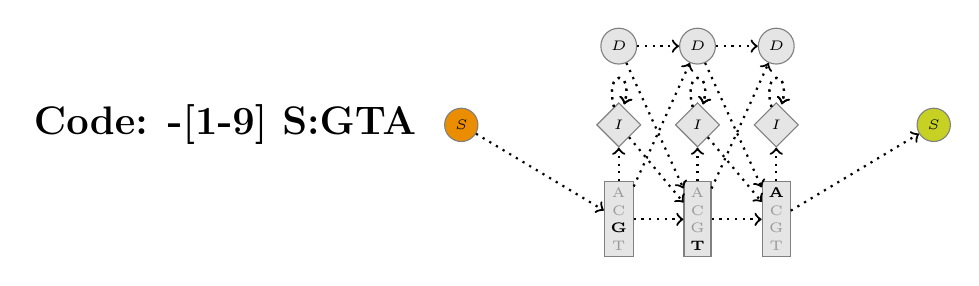
\begin{tikzpicture}
 \tiny
  \node  at (-6,0)  [font=\Large,style={align=center}] () {{\bf Code: -[1-9] S:GTA}};
 
 \node[Dstate,fill=orange] (START) at (-3,0){$S$};
 
\node[Dstate,fill=yellowgreen] (END) at (3,0){$S$};
 
\begin{scope}[shift={(-1,0)}];
\node[Dstate] (d1) at (0,1){$D$};
\node[Istate] (i1) at (0,0){$I$};
\node[Mstate] (m1) at (0,-1.2){\shortstack{ {\color{black!40}A}\\   {\color{black!40}C}\\  {\bf G}\\   {\color{black!40}T}} };



\node[Dstate] (d2) at (1,1){$D$};
\node[Istate] (i2) at (1,0){$I$};
\node[Mstate] (m2) at (1,-1.2){\shortstack{ {\color{black!40}A}\\   {\color{black!40}C}\\   {\color{black!40}G}\\   {\bf T}} };


\node[Dstate] (d3) at (2,1){$D$};
\node[Istate] (i3) at (2,-0){$I$};
\node[Mstate] (m3) at (2,-1.2){\shortstack{ {\bf A}\\   {\color{black!40}C}\\   {\color{black!40}G}\\   {\color{black!40}T}} };
\end{scope}

\path
(START)  edge [lightedge] (m1) 


(m3)  edge [lightedge] (END) 

(m1) edge [lightedge] (m2) 
(m1) edge [lightedge] (d2) 
(m1) edge [lightedge] (i1)
   
(i1) edge [lightedge,loop above] ()
(i1) edge  [lightedge] (m2)
(i1) edge [lightedge, loop above] ()
(d1) edge  [lightedge,->] (d2)
(d1) edge  [lightedge,->] (m2)

(m2) edge [lightedge] (m3) 
(m2) edge [lightedge] (d3) 
(m2) edge [lightedge] (i2)
   
(i2) edge [lightedge,loop above] ()
(i2) edge  [lightedge] (m3)
(i2) edge [lightedge, loop above] ()
(d2) edge  [lightedge,->] (d3)
(d2) edge  [lightedge,->] (m3)


(m3) edge [lightedge] (i3)
   
(i3) edge [lightedge,loop above] ()

(i3) edge [lightedge, loop above] ();




\end{tikzpicture}
\end{figure}

\section{Partial}
This segment is used to model sequences that may only be partially present at the 5` or 3` end of the read. The transition probabilities (orange and blue) are set automatically based on the length distribution of {\bf exactly} matching adapters.\\

\begin{figure}[H]
\centering
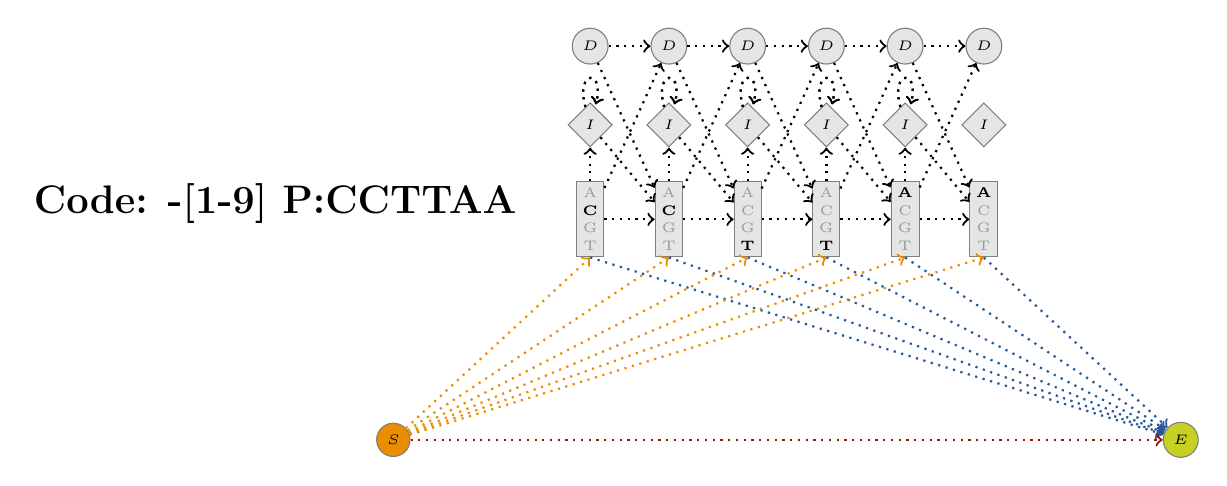
\begin{tikzpicture}
 \tiny
  \node  at (-2.5,1)  [font=\Large,style={align=center}] () {{\bf Code: -[1-9] P:CCTTAA}};
 
 \node[Dstate,fill=orange] (START) at (-1,-2){$S$};
\begin{scope}[shift={(1.5,2)}];

%CCTTAAGG
\node[Dstate] (dl1) at (0,1){$D$};
\node[Istate] (il1) at (0,0){$I$};
\node[Mstate] (ml1) at (0,-1.2){\shortstack{ {\color{black!40}A}\\  {\bf C} \\   {\color{black!40}G}\\ {\color{black!40}T}} };

\node[Dstate] (dl2) at (1,1){$D$};
\node[Istate] (il2) at (1,0){$I$};
\node[Mstate] (ml2) at (1,-1.2){\shortstack{ {\color{black!40}A}\\   {\bf C}\\   {\color{black!40}G}\\   {\color{black!40}T}} };

\node[Dstate] (dl3) at (2,1){$D$};
\node[Istate] (il3) at (2,-0){$I$};
\node[Mstate] (ml3) at (2,-1.2){\shortstack{ {\color{black!40}A}\\   {\color{black!40}C}\\   {\color{black!40}G}\\   {\bf T}} };

\node[Dstate] (dl4) at (3,1){$D$};
\node[Istate] (il4) at (3,0){$I$};
\node[Mstate] (ml4) at (3,-1.2){\shortstack{ {\color{black!40}A}\\   {\color{black!40}C}\\   {\color{black!40}G}\\   {\bf T}} };

\node[Dstate] (dl5) at (4,1){$D$};
\node[Istate] (il5) at (4,0){$I$};
\node[Mstate] (ml5) at (4,-1.2){\shortstack{ {\bf A}\\   {\color{black!40}C}\\   {\color{black!40}G}\\   {\color{black!40}T}} };

\node[Dstate] (dl6) at (5,1){$D$};
\node[Istate] (il6) at (5,-0){$I$};
\node[Mstate] (ml6) at (5,-1.2){\shortstack{ {\bf A}\\   {\color{black!40}C}\\   {\color{black!40}G}\\   {\color{black!40}T}} };
\end{scope}

\begin{scope}[shift={(9,-2)}];
\node[Dstate,fill=yellowgreen] (END) at (0,0){$E$};
\end{scope}


 \path

%(START)  edge [lightedge] (ml1)
(ml1) edge [lightedge] (ml2) 
(ml1) edge [lightedge] (dl2) 
(ml1) edge [lightedge] (il1)
   
(il1) edge [lightedge,loop above] ()
(il1) edge  [lightedge] (ml2)
(il1) edge [lightedge, loop above] ()
(dl1) edge  [lightedge,->] (dl2)
(dl1) edge  [lightedge,->] (ml2)

(ml2) edge [lightedge] (ml3) 
(ml2) edge [lightedge] (dl3) 
(ml2) edge [lightedge] (il2)
   
(il2) edge [lightedge,loop above] ()
(il2) edge  [lightedge] (ml3)
(il2) edge [lightedge, loop above] ()
(dl2) edge  [lightedge,->] (dl3)
(dl2) edge  [lightedge,->] (ml3)


(ml3) edge [lightedge] (ml4) 
(ml3) edge [lightedge] (dl4) 
(ml3) edge [lightedge] (il3)
   
(il3) edge [lightedge,loop above] ()
(il3) edge  [lightedge] (ml4)
(il3) edge [lightedge, loop above] ()
(dl3) edge  [lightedge,->] (dl4)
(dl3) edge  [lightedge,->] (ml4)


(ml4) edge [lightedge] (ml5) 
(ml4) edge [lightedge] (dl5) 
(ml4) edge [lightedge] (il4)
   
(il4) edge [lightedge,loop above] ()
(il4) edge  [lightedge] (ml5)
(il4) edge [lightedge, loop above] ()
(dl4) edge  [lightedge,->] (dl5)
(dl4) edge  [lightedge,->] (ml5)



(ml5) edge [lightedge] (ml6) 
(ml5) edge [lightedge] (dl6) 
(ml5) edge [lightedge] (il5)
   
(il5) edge [lightedge,loop above] ()
(il5) edge  [lightedge] (ml6)
(il5) edge [lightedge, loop above] ()
(dl5) edge  [lightedge,->] (dl6)
(dl5) edge  [lightedge,->] (ml6)


(ml1.south)edge [blue,lightedge] (END)
(ml2.south)edge [blue,lightedge] (END)
(ml3.south)edge [blue,lightedge] (END)
(ml4.south)edge [blue,lightedge] (END)
(ml5.south)edge [blue,lightedge] (END)
(ml6.south)edge [blue,lightedge] (END)

(START)edge [orange,lightedge] (ml1.south)
(START)edge [orange,lightedge] (ml2.south)
(START)edge [orange,lightedge] (ml3.south)
(START)edge [orange,lightedge] (ml4.south)
(START)edge [orange,lightedge] (ml5.south)
(START)edge [orange,lightedge] (ml6.south)
(START)edge [winered,lightedge] (END)

;

\end{tikzpicture}
\end{figure}






\chapter{Algorithm}

\section{Sequence scoring} 

In short read mapping the mapping quality Q reflects the confidence we have in one particular mapping location over all others \cite{li2008mapping}. Analogously, TagDust2 compares the probability of each read matching to the user specified HMM to the total summed probability including a random model:

\begin{equation}\label{eq:main}
P = 1 - \frac{P(x|M)*V}{P(x|M) + P(x|R)}
\end{equation} 

where $P(x|M)$ is the total summed probability of a read matching the model derived by the forward algorithm and $P(x|R)$ is the probability of the read give a random zero order Markov model. $V$ represents the fraction of $P(x|M)$ corresponding to the most likely barcode sequence. It is derived by using the backward and forward algorithm at each mutual exclusive transition:

\begin{equation}
	V = \max_j \left( \frac{f_s(i)   a_{s,m_j} e_{m_j}(x+1) b_{m_j}(i+1)}{\sum\limits_{\pi} P(x,\pi | M )}\right)
\end{equation}

where $ a_{s,m_j}$ is the transition from a silent to the first match state $m_j$ of a HMM modeling a barcode.  
 

\section{Threshold selection} 

In versions prior to 2.11 users could specify a threshold with the -q option. Unfortunately, when using simple read architectures (48 3bp barcodes followed by a read) often no reads obtained a reasonable $P$ (equation \ref{eq:main}). 

TagDust now simulated reads based on the model and random model and selects a threshold automatically giving the best specificity plus sensitivity.  

\section{Implementation} 

Internally, TagDust uses a full profile HMM for each building block. We simply set some transition probabilities to zero to emulate different models. For example the read building block 'R' is implemented as a profile HMM with one column and transitions directly to and from the insertion state.
This is fairly inefficient as the dynamic programming code still needs to evaluate all possible transitions, even those we know in advance have a probability of zero. In future I might do something about this. 

\section{Optimal accuracy decoding} 

To obtain the most probably labeling of the sequence, we employ the optimal accuracy decoding algorithm as described in \citep{Kall:2005vg}. To apply this algorithm to our problem define the label probability of a nucleotide by the summed posterior label probabilities of states belonging to a particular HMM building block. A secondary dynamic programming algorithm is used to determine the path with the maximal label probability, constrained by the global HMM architecture. The label probabilities are essentially used as a substitution matrix while the architecture is enforced by the equivalent of gap penalties. 

If fingerprints are present TagDust checks at this stage if the length after decoding matches the users input. If not the read is discarded. 



%\chapter{Acknowledgements }


\begin{comment}
\chapter{hshsaer}
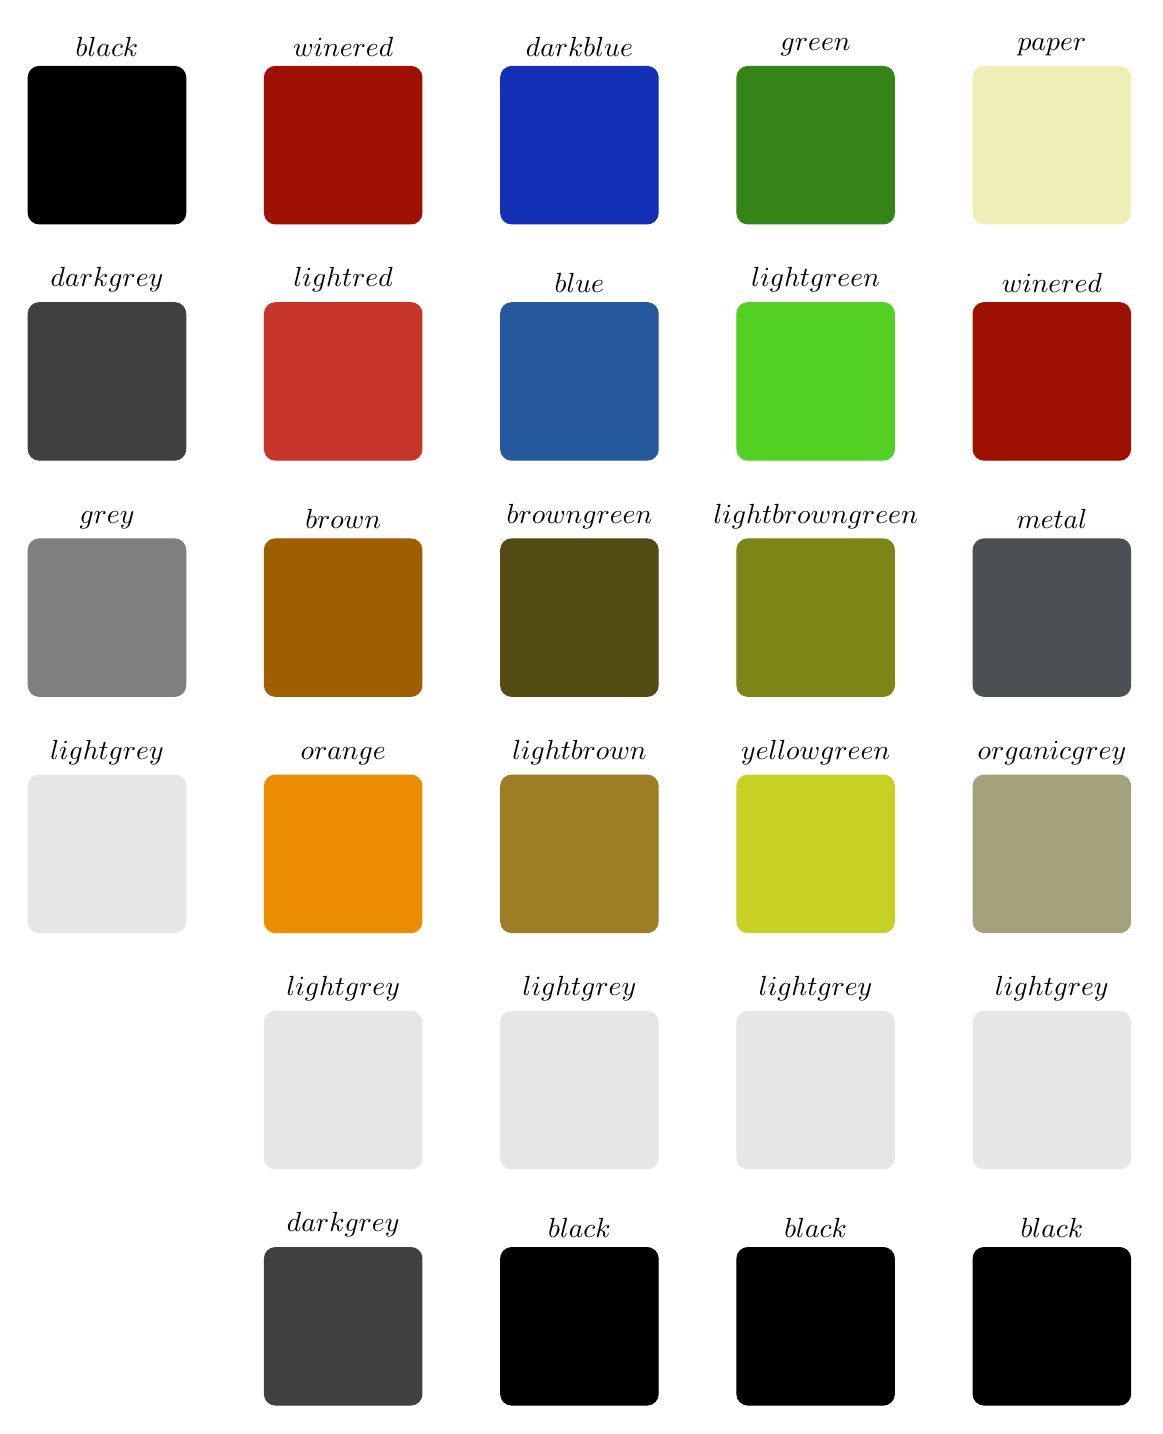
\begin{tikzpicture}[]
%\definecolor{black}{RGB}{0,0,0}
%\definecolor{darkgrey}{RGB}{64,64,64}
%\definecolor{grey}{RGB}{127,127,127}
%\definecolor{lightgrey}{RGB}{230,230,230}
\node [draw=black, fill=black,rounded corners=4pt,draw,rectangle,minimum width=2cm,minimum height=2cm,label=$black$] at (0,0) {};

\node [draw=darkgrey, fill=darkgrey,rounded corners=4pt,draw,rectangle,minimum width=2cm,minimum height=2cm,label=$darkgrey$] at (0,-3) {};

\node [draw=grey, fill=grey,rounded corners=4pt,draw,rectangle,minimum width=2cm,minimum height=2cm,label=$grey$] at (0,-6) {};

\node [draw=lightgrey, fill=lightgrey,rounded corners=4pt,draw,rectangle,minimum width=2cm,minimum height=2cm,label=$lightgrey$] at (0,-9) {};

%\definecolor{winered}{RGB}{158,16,0}
%\definecolor{ligthred}{RGB}{199,53,42}
%\definecolor{brown}{RGB}{158,95,0}
%\definecolor{orange}{RGB}{235,141,0}
\begin{scope}[shift={(3,0)}];
\node [draw=winered, fill=winered,rounded corners=4pt,draw,rectangle,minimum width=2cm,minimum height=2cm,label=$winered$] at (0,0) {};

\node [draw=lightred, fill=lightred,rounded corners=4pt,draw,rectangle,minimum width=2cm,minimum height=2cm,label=$lightred$] at (0,-3) {};

\node [draw=brown, fill=brown,rounded corners=4pt,draw,rectangle,minimum width=2cm,minimum height=2cm,label=$brown$] at (0,-6) {};

\node [draw=orange, fill=orange,rounded corners=4pt,draw,rectangle,minimum width=2cm,minimum height=2cm,label=$orange$] at (0,-9) {};

\node [draw=lightgrey, fill=lightgrey,rounded corners=4pt,draw,rectangle,minimum width=2cm,minimum height=2cm,label=$lightgrey$] at (0,-12) {};

\node [draw=darkgrey, fill=darkgrey,rounded corners=4pt,draw,rectangle,minimum width=2cm,minimum height=2cm,label=$darkgrey$] at (0,-15) {};

\end{scope}


%\definecolor{darkblue}{RGB}{19,48,182}

%\definecolor{blue}{RGB}{36,89,158}
%\definecolor{browngreen}{RGB}{82,75,19}
%\definecolor{lightbrown}{RGB}{158,126,36}

\begin{scope}[shift={(6,0)}];
\node [draw=darkblue, fill=darkblue,rounded corners=4pt,draw,rectangle,minimum width=2cm,minimum height=2cm,label=$darkblue$] at (0,0) {};

\node [draw=blue, fill=blue,rounded corners=4pt,draw,rectangle,minimum width=2cm,minimum height=2cm,label=$blue$] at (0,-3) {};

\node [draw=browngreen, fill=browngreen,rounded corners=4pt,draw,rectangle,minimum width=2cm,minimum height=2cm,label=$browngreen$] at (0,-6) {};

\node [draw=lightbrown, fill=lightbrown,rounded corners=4pt,draw,rectangle,minimum width=2cm,minimum height=2cm,label=$lightbrown$] at (0,-9) {};

\node [draw=lightgrey, fill=lightgrey,rounded corners=4pt,draw,rectangle,minimum width=2cm,minimum height=2cm,label=$lightgrey$] at (0,-12) {};

\node [draw=black, fill=black,rounded corners=4pt,draw,rectangle,minimum width=2cm,minimum height=2cm,label=$black$] at (0,-15) {};

\end{scope}

%\definecolor{green}{RGB}{52,132,23}
%\definecolor{lightgreen}{RGB}{82,209,36}
%\definecolor{lightbrowngreen}{RGB}{125,133,23}
%\definecolor{yellowgreen}{RGB}{198,209,36}


\begin{scope}[shift={(9,0)}];
\node [draw=green, fill=green,rounded corners=4pt,draw,rectangle,minimum width=2cm,minimum height=2cm,label=$green$] at (0,0) {};

\node [draw=lightgreen, fill=lightgreen,rounded corners=4pt,draw,rectangle,minimum width=2cm,minimum height=2cm,label=$lightgreen$] at (0,-3) {};

\node [draw=lightbrowngreen, fill=lightbrowngreen,rounded corners=4pt,draw,rectangle,minimum width=2cm,minimum height=2cm,label=$lightbrowngreen$] at (0,-6) {};

\node [draw=yellowgreen, fill=yellowgreen,rounded corners=4pt,draw,rectangle,minimum width=2cm,minimum height=2cm,label=$yellowgreen$] at (0,-9) {};

\node [draw=lightgrey, fill=lightgrey,rounded corners=4pt,draw,rectangle,minimum width=2cm,minimum height=2cm,label=$lightgrey$] at (0,-12) {};

\node [draw=black, fill=black,rounded corners=4pt,draw,rectangle,minimum width=2cm,minimum height=2cm,label=$black$] at (0,-15) {};

\end{scope}

%\definecolor{paper}{RGB}{240,238,183}
%\definecolor{organicgrey}{RGB}{163,162,124}
%\definecolor{metal}{RGB}{75,81,82}

\begin{scope}[shift={(12,0)}];
\node [draw=paper, fill=paper,rounded corners=4pt,draw,rectangle,minimum width=2cm,minimum height=2cm,label=$paper$] at (0,0) {};

\node [draw=winered, fill=winered,rounded corners=4pt,draw,rectangle,minimum width=2cm,minimum height=2cm,label=$winered$] at (0,-3) {};

\node [draw=metal, fill=metal,rounded corners=4pt,draw,rectangle,minimum width=2cm,minimum height=2cm,label=$metal$] at (0,-6) {};

\node [draw=organicgrey, fill=organicgrey,rounded corners=4pt,draw,rectangle,minimum width=2cm,minimum height=2cm,label=$organicgrey$] at (0,-9) {};

\node [draw=lightgrey, fill=lightgrey,rounded corners=4pt,draw,rectangle,minimum width=2cm,minimum height=2cm,label=$lightgrey$] at (0,-12) {};

\node [draw=black, fill=black,rounded corners=4pt,draw,rectangle,minimum width=2cm,minimum height=2cm,label=$black$] at (0,-15) {};


\end{scope}


%\draw[rounded corners=4pt,draw=hgrey, fill=hlightblue] (0,-6)	rectangle (+1,+1);
%\draw[rounded corners=4pt,draw=hgrey, fill=hlightblue] (0,-9)	rectangle (+1,+1);




\end{tikzpicture}
\end{comment}
\newpage
  
%-----------------------------------------------------------
\addcontentsline{toc}{chapter}{\numberline{}Bibliography}
\bibliographystyle{plain}
\bibliography{ref}


%-----------------------------------------------------------
%\appendix
%
%\chapter{Long proofs}\label{app:proofs} An Appendix is a good place
%to put lengthy proofs that must be included but would impede the
%flow if placed in the main text.
%\section{Proof of theorem}\label{pf:angels}
%By inspection.

%-----------------------------------------------------------
\end{document}
